% THIS DOCUMENT IS TAILORED TO REQUIREMENTS FOR SCIENTIFIC COMPUTING.  IT SHOULDN'T
% BE USED FOR NON-SCIENTIFIC COMPUTING PROJECTS
\documentclass[12pt]{article}

\usepackage{amsmath, mathtools}
\usepackage{amsfonts}
\usepackage{amssymb}
\usepackage{graphicx}
\usepackage{colortbl}
\usepackage{xr}
\usepackage{hyperref}
\usepackage{longtable}
\usepackage{xfrac}
\usepackage{tabularx}
\usepackage{float}
\usepackage{siunitx}
\usepackage{booktabs}
\usepackage{caption}
\usepackage{pdflscape}
\usepackage{afterpage}

\usepackage[round]{natbib}

%\usepackage{refcheck}

\hypersetup{
    bookmarks=true,         % show bookmarks bar?
      colorlinks=true,       % false: boxed links; true: colored links
    linkcolor=red,          % color of internal links (change box color with linkbordercolor)
    citecolor=green,        % color of links to bibliography
    filecolor=magenta,      % color of file links
    urlcolor=cyan           % color of external links
}

%% Comments

\usepackage{color}

\newif\ifcomments\commentstrue %displays comments
%\newif\ifcomments\commentsfalse %so that comments do not display

\ifcomments
\newcommand{\authornote}[3]{\textcolor{#1}{[#3 ---#2]}}
\newcommand{\todo}[1]{\textcolor{red}{[TODO: #1]}}
\else
\newcommand{\authornote}[3]{}
\newcommand{\todo}[1]{}
\fi

\newcommand{\wss}[1]{\authornote{blue}{SS}{#1}} 
\newcommand{\plt}[1]{\authornote{magenta}{TPLT}{#1}} %For explanation of the template
\newcommand{\an}[1]{\authornote{cyan}{Author}{#1}}

%% Common Parts

\newcommand{\progname}{ProgName} % PUT YOUR PROGRAM NAME HERE
\newcommand{\authname}{Team \#, Team Name
\\ Student 1 name
\\ Student 2 name
\\ Student 3 name
\\ Student 4 name} % AUTHOR NAMES                  

\usepackage{hyperref}
    \hypersetup{colorlinks=true, linkcolor=blue, citecolor=blue, filecolor=blue,
                urlcolor=blue, unicode=false}
    \urlstyle{same}
                                


% For easy change of table widths
\newcommand{\colZwidth}{1.0\textwidth}
\newcommand{\colAwidth}{0.13\textwidth}
\newcommand{\colBwidth}{0.82\textwidth}
\newcommand{\colCwidth}{0.1\textwidth}
\newcommand{\colDwidth}{0.05\textwidth}
\newcommand{\colEwidth}{0.8\textwidth}
\newcommand{\colFwidth}{0.17\textwidth}
\newcommand{\colGwidth}{0.5\textwidth}
\newcommand{\colHwidth}{0.28\textwidth}

% Used so that cross-references have a meaningful prefix
\newcounter{defnum} %Definition Number
\newcommand{\dthedefnum}{GD\thedefnum}
\newcommand{\dref}[1]{GD\ref{#1}}
\newcounter{datadefnum} %Datadefinition Number
\newcommand{\ddthedatadefnum}{DD\thedatadefnum}
\newcommand{\ddref}[1]{DD\ref{#1}}
\newcounter{theorynum} %Theory Number
\newcommand{\tthetheorynum}{TM\thetheorynum}
\newcommand{\tref}[1]{TM\ref{#1}}
\newcounter{tablenum} %Table Number
\newcommand{\tbthetablenum}{TB\thetablenum}
\newcommand{\tbref}[1]{TB\ref{#1}}
\newcounter{assumpnum} %Assumption Number
\newcommand{\atheassumpnum}{A\theassumpnum}
\newcommand{\aref}[1]{A\ref{#1}}
\newcounter{goalnum} %Goal Number
\newcommand{\gthegoalnum}{GS\thegoalnum}
\newcommand{\gsref}[1]{GS\ref{#1}}
\newcounter{instnum} %Instance Number
\newcommand{\itheinstnum}{IM\theinstnum}
\newcommand{\iref}[1]{IM\ref{#1}}
\newcounter{reqnum} %Requirement Number
\newcommand{\rthereqnum}{R\thereqnum}
\newcommand{\rref}[1]{R\ref{#1}}
\newcounter{nfrnum} %NFR Number
\newcommand{\rthenfrnum}{NFR\thenfrnum}
\newcommand{\nfrref}[1]{NFR\ref{#1}}
\newcounter{lcnum} %Likely change number
\newcommand{\lthelcnum}{LC\thelcnum}
\newcommand{\lcref}[1]{LC\ref{#1}}

\usepackage{fullpage}

\newcommand{\deftheory}[9][Not Applicable]
{
\newpage
\noindent \rule{\textwidth}{0.5mm}

\paragraph{RefName: } \textbf{#2} \phantomsection 
\label{#2}

\paragraph{Label:} #3

\noindent \rule{\textwidth}{0.5mm}

\paragraph{Equation:}

#4

\paragraph{Description:}

#5

\paragraph{Notes:}

#6

\paragraph{Source:}

#7

\paragraph{Ref.\ By:}

#8

\paragraph{Preconditions for \hyperref[#2]{#2}:}
\label{#2_precond}

#9

\paragraph{Derivation for \hyperref[#2]{#2}:}
\label{#2_deriv}

#1

\noindent \rule{\textwidth}{0.5mm}

}

\begin{document}

\title{Software Requirements Specification for BrainInsight3D: 3D fMRI
  Visualization \& Segmentation}
\author{Nada Elmasry}
\date{\today}

\maketitle

~\newpage

\pagenumbering{roman}

\tableofcontents

~\newpage

\section*{Revision History}

\begin{tabularx}{\textwidth}{p{3cm}p{2cm}X}
  \toprule {\bf Date} & {\bf Version} & {\bf Notes}         \\
  \midrule
  Feb 5               & 1.0           & Intial SRS Document \\
  \bottomrule
\end{tabularx}

~\\


~\newpage

\section{Reference Material}

This section records information for easy reference.

\subsection{Table of Units}

Throughout this document SI (Syst\`{e}me International d'Unit\'{e}s) is employed
as the unit system.  In addition to the basic units, several derived units are
used as described below.  For each unit, the symbol is given followed by a
description of the unit and the SI name.
~\newline

\renewcommand{\arraystretch}{1.2}
%\begin{table}[ht]
\noindent \begin{tabular}{l l l}
  \toprule
  \textbf{symbol} & \textbf{unit} & \textbf{SI}                       \\
  \midrule
  \si{\metre}     & length        & metre                             \\
  \si{\kilogram}  & mass          & kilogram                          \\
  \si{\second}    & time          & second                            \\
  \si{\celsius}   & temperature   & centigrade                        \\
  \si{\joule}     & energy        & joule                             \\
  \si{\watt}      & power         & watt (W = \si{\joule\per\second}) \\
  \bottomrule
\end{tabular}
%	\caption{Provide a caption}
%\end{table}


\subsection{Table of Symbols}

The table that follows summarizes the symbols used in this document along with
their units.  The choice of symbols was made to be consistent with the heat
transfer literature and with existing documentation for solar water heating
systems.  The symbols are listed in alphabetical order.

\renewcommand{\arraystretch}{1.2}
%\noindent \begin{tabularx}{1.0\textwidth}{l l X}
\noindent \begin{longtable*}{l l p{12cm}} \toprule
  \textbf{symbol} & \textbf{unit} & \textbf{description}\\
  \midrule
  $A_C$ & \si[per-mode=symbol] {\square\metre} & coil surface area
  \\
  $A_\text{in}$ & \si[per-mode=symbol] {\square\metre} & surface area over
  which heat is transferred in
  \\
  \bottomrule
\end{longtable*}
\plt{Use your problems actual symbols.  The si package is a good idea to use for
  units.}

\subsection{Abbreviations and Acronyms}

\renewcommand{\arraystretch}{1.2}
\begin{tabular}{l l}
  \toprule
  \textbf{symbol} & \textbf{description}                                                     \\
  \midrule
  A               & Assumption                                                               \\
  DD              & Data Definition                                                          \\
  GD              & General Definition                                                       \\
  GS              & Goal Statement                                                           \\
  IM              & Instance Model                                                           \\
  LC              & Likely Change                                                            \\
  PS              & Physical System Description                                              \\
  R               & Requirement                                                              \\
  SRS             & Software Requirements Specification                                      \\
  \progname{}     & \plt{put an expanded version of your program name here (as appropriate)} \\
  TM              & Theoretical Model                                                        \\
  \bottomrule
\end{tabular}\\


\newpage

\pagenumbering{arabic}


\section{Introduction}


This document provides the software specification requirements(SRS) for the
BrainInsight 3D project. The project offers 3D and 2D visualization and segmentation
of fMRI brain scans with time and functional activity tracking in 2D through a
web application that enables high-resolution visualization and segmentation.

This introductory section explains the purpose of this document, the organization of
the document,the project scope of requirements, and the characteristics of the intended
reader.

\subsection{Purpose of Document}

The purpose of this document is to provide the reader with a thorough understanding
of what the project does. The document contains all the definitions, theoritical and
instance models, inputs, outputs, assumptions, and goals of the project. After reading
the document the reader should be able to define the project and have a visual imagery
of what the project represents.
\subsection{Scope of Requirements}

Thr scope of requirements of the project covers mainly two parts:
1. Visualization: the project's software will visualize fMRI scans into 3D volumes,
and 2D slices representing the anatomical coordinate system used by the fMRI scan.
2. Segmentation: the project's software can perform anatomical segmentation of 3D volumes into voxels,
and on 2D slices into pixels.

The user requirements are to be able to input the correct data type into the project's
software, manipulate the user interface to change visualization settings, and to interpret
the results of the visualization and segmentation.


\subsection{Characteristics of Intended Reader} \label{sec_IntendedReader}

The readers of the SRS should have taken introductory courses in linear algebra, anatomy,
and computer vision to be able to understand the mathematical notations, co-ordinate systems,
and instance models provided in the SRS document.It would be beneficial if the reader has a
background in software engineering in order to better visualize the project scope and requirements,
however, it is not a hard requirement.

\subsection{Organization of Document}

The organization of this document follows the template for an SRS for
scientific computing software proposed by \cite{Koothoor2013} and
\cite{SmithAndLai2005}. The presentation follows the standard pattern of presenting goals, theories, definitions and
assumptions. The goal statements are refined to the theoretical models, and
theoretical models to the instance models. For readers that would like a more bottom-up
approach, they can start reading the instance models in Section
\ref{sssec:im} and trace back to find any additional information they require.


\section{General System Description}
This section provides general information about the system, identifies the
interfaces between the system and its environment, and describes the user
characteristics and the system constraints.


\subsection{System Context}

Figure \ref{SystemContext} shows the system context.  A circle represents an
external entity outside the software, the user in this case.  A rectangle
represents the software system itself.  Arrows are used to show the data
flow between the system and its environment.
\newline\newline\newline

\begin{figure}[h!]
  \begin{center}
    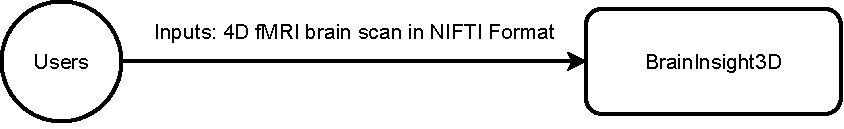
\includegraphics[width=0.6\textwidth]{SystemContext}
    \caption{System Context}
    \label{SystemContext}
  \end{center}
\end{figure}


\begin{itemize}
  \item User Responsibilities:
        \begin{itemize}
          \item Provide the correct input data to the program
          \item make sure the input meets the required assumptions
          \item Verify that the output visualization and segmentation
                results meet their requirements.
          \item Use the provided options in the program to obtain their
                desired visualization.
        \end{itemize}
  \item \progname{} Responsibilities:
        \begin{itemize}
          \item Correctly visualize 3D volumes
          \item Correctly visualize 2D slices according to the anatomical
                coordinate system explained in \ref{Terminology and  Definitions}.
          \item Correctly perform segmentation of 3D fMRI volumes into the brain
                anatomical regions  explained in \ref{Terminology and  Definitions}.
          \item Provide the user input options to be able to choose wether to visualize
                the complete 3D volume or a sub-volume, and to be able to visualize 2D slices and
                segemntation results simultaneously across the time frame of the fMRI scan.
        \end{itemize}
\end{itemize}

\subsection{User Characteristics} \label{SecUserCharacteristics}

The intended user of BrainInsight3D should have taken college level introductory
courses in Linear Algebra and Anatomy.

\subsection{System Constraints}
There are no system constraints for BrainInsight3D.

\section{Specific System Description}

This section first presents the problem description, which gives a high-level
view of the problem to be solved.  This is followed by the solution characteristics
specification, which presents the assumptions, theories, definitions and finally
the instance models.

\subsection{Problem Description} \label{Sec_pd}

BrainInsight3D is designed to offer high-resolution visualization and anatomical
segmentation of fMRI brain scans, enabling the tracking of changes across various
time frames within the scan.

\subsubsection{Co-ordinate Systems}
the purpose of this section is to provide the reader with the knowledge of the co-ordinate systems
required to understand and work with medical images. \ref*{Nejad2017}

\paragraph*{World Coordinate System}

World Coordinate system is a Cartesian coordinate system in which a model (e.g. a MRI scanner or a patient) is positioned.
While each model has it's own coordinate system, all models must be transformed into world coordinate system for accurate model interaction.
\begin{figure}[hbpt!]
  \centering
  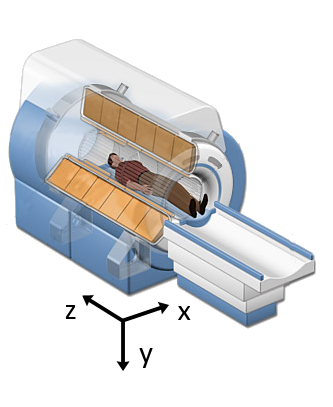
\includegraphics[width=50mm]{world-coordinate-sytem.png}
  \caption{visualization of MRI machine placed in World Coordinate System~\cite{SlicerWikiCoordinateSystems}}
  \label{worldcoordfMRI}
\end{figure}



\paragraph*{Anatomical Coordinate System}
The Anatomical Coordinate System is a 3D right-handed coordinate system that describes human anatomy through three planes:\cite{SlicerWikiCoordinateSystems} \cite{Nejad2017}
\begin{itemize}
  \item \textbf{Axial/Transverse plane}: is parallel to the ground and separates the head (Superior) from the feet (Inferior).
  \item \textbf{Coronal/Frontal plane}: is perpendicular to the ground and separates the front from (Anterior) the back (Posterior).
  \item \textbf{Sagittal/Median plane}: divides the body to left and right parts.
\end{itemize}
\begin{figure}[hbpt!]
  \centering
  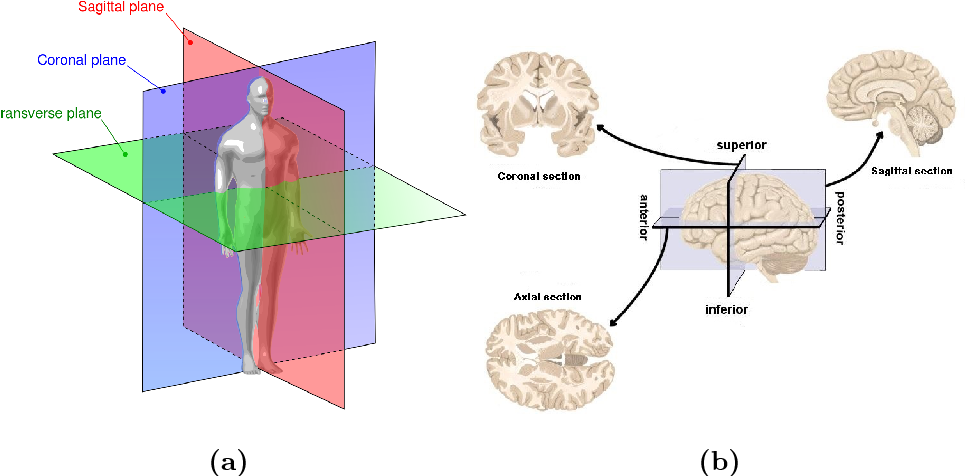
\includegraphics[width=70mm]{anatomical-coordinate-sytem-fmri.png}
  \caption{Anatomical Coordinate System Axes and Planes~\cite{Asaei2015BrainML}}
  \label{anatomicalcoordfMRI}
\end{figure}

Medical applications follow an anatomical coordinate system to store voxels in sequences using different definitions. The most common basis are:
\begin{itemize}
  \item  \textbf{Left-Posterior-Superior(LPS) System}: In this system, voxels are ordered
        from left to right in a row, rows are ordered from anterior to posterior, and slices are
        stored from inferior to superior. LPS System is commonly used in DICOM images.
  \item  \textbf{Right, Anterior, Superior(RAS) System}: In this system, voxels are ordered
        from right to left in a row, rows are ordered from posterior to anterior, and slices are
        stored from inferior to superior. RAS System is commonly used in NIfTI images and will be used for this project.
\end{itemize}
\paragraph*{Image Coordinate System}
In our project we will be utilizing the OpenCV Python library.In OpenCV image coordinate
system, x-axis increases from left to right, y-axis increases from top to bottom, and z-axis
from forward to backward.
\begin{figure}[hbpt!]
  \centering
  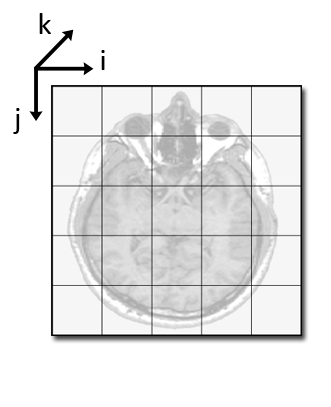
\includegraphics[width=50mm]{image-coordinate-system.png}
  \caption{Image Coordinate System used in OpenCV Python~\cite{SlicerWikiCoordinateSystems}}
  \label{imagecoordfMRI}
\end{figure}





\subsubsection{Brain Segmentation}
Segmentation precisely divides an object into related entities, each representing specific locations or meanings.
In medical imaging, it's crucial for extracting key data from scans, including organs, tumors, tissues, or nerves.
Brain imaging relies heavily on segmentation to gain insight into the brain's structure and function.
There are two primary types: functional segmentation, which focuses on brain activity, and anatomical segmentation, which details the brain's physical structure.

\paragraph*{Anatomical Segmentation}
Anatomical segmentation is a crucial process in neuroimaging that consists of dividing the brain into structurally distinct areas based on MRI scans,
identifying regions such as gray matter, white matter, and cerebrospinal fluid. This segmentation is essential for a wide range of neuroscience studies,
enabling researchers to precisely localize brain activity, assess changes in brain structure over time, or study the anatomical differences between populations.
The process of anatomical segmentation has been significantly advanced by the use of deep learning techniques, notably U-Net and Convolutional Neural Networks (CNNs).
These methods have proven effective in handling the complexity of brain structures, providing high accuracy in segmentation tasks.


\begin{figure}[hbpt!]
  \centering
  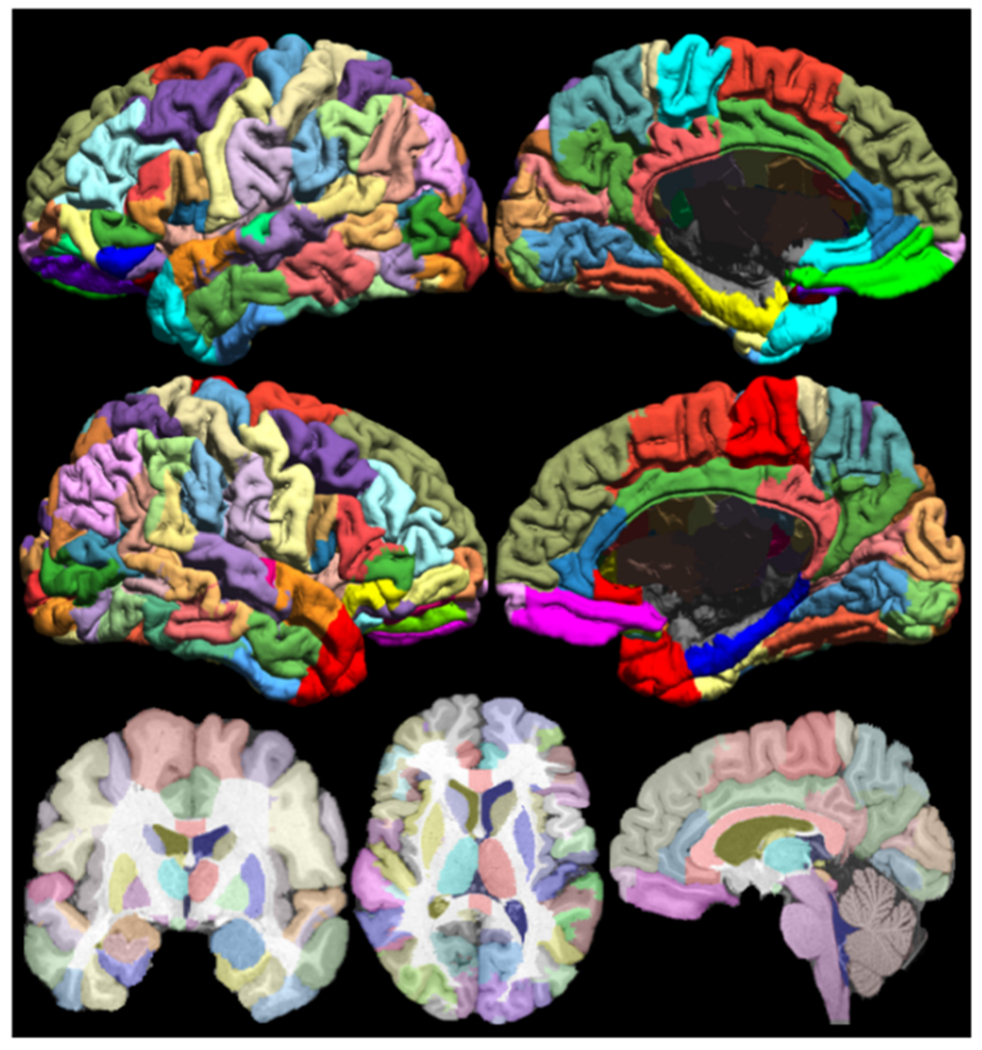
\includegraphics[width=50mm]{anatomical-seg-fmri.jpg}
  \caption{Results of anatomical segmentation on fMRI scan~\cite{joshi2022hybrid}}
  \label{anatomicalsegfMRI}
\end{figure}

\paragraph*{Functional Segmentation}

Functional segmentation is a process that categorizes the brain into regions
that exhibit similar patterns of activity, either during specific tasks or in a
resting state. This division is typically achieved through the application of
statistical techniques such as Independent Component Analysis (ICA) or through
machine learning approaches like K-Nearest Neighbors (KNNs).This approach is crucial for understanding
brain connectivity and function, offering insights into neural interactions
and the impact of disorders or stimuli on the brain.

\begin{figure}[hbpt!]
  \centering
  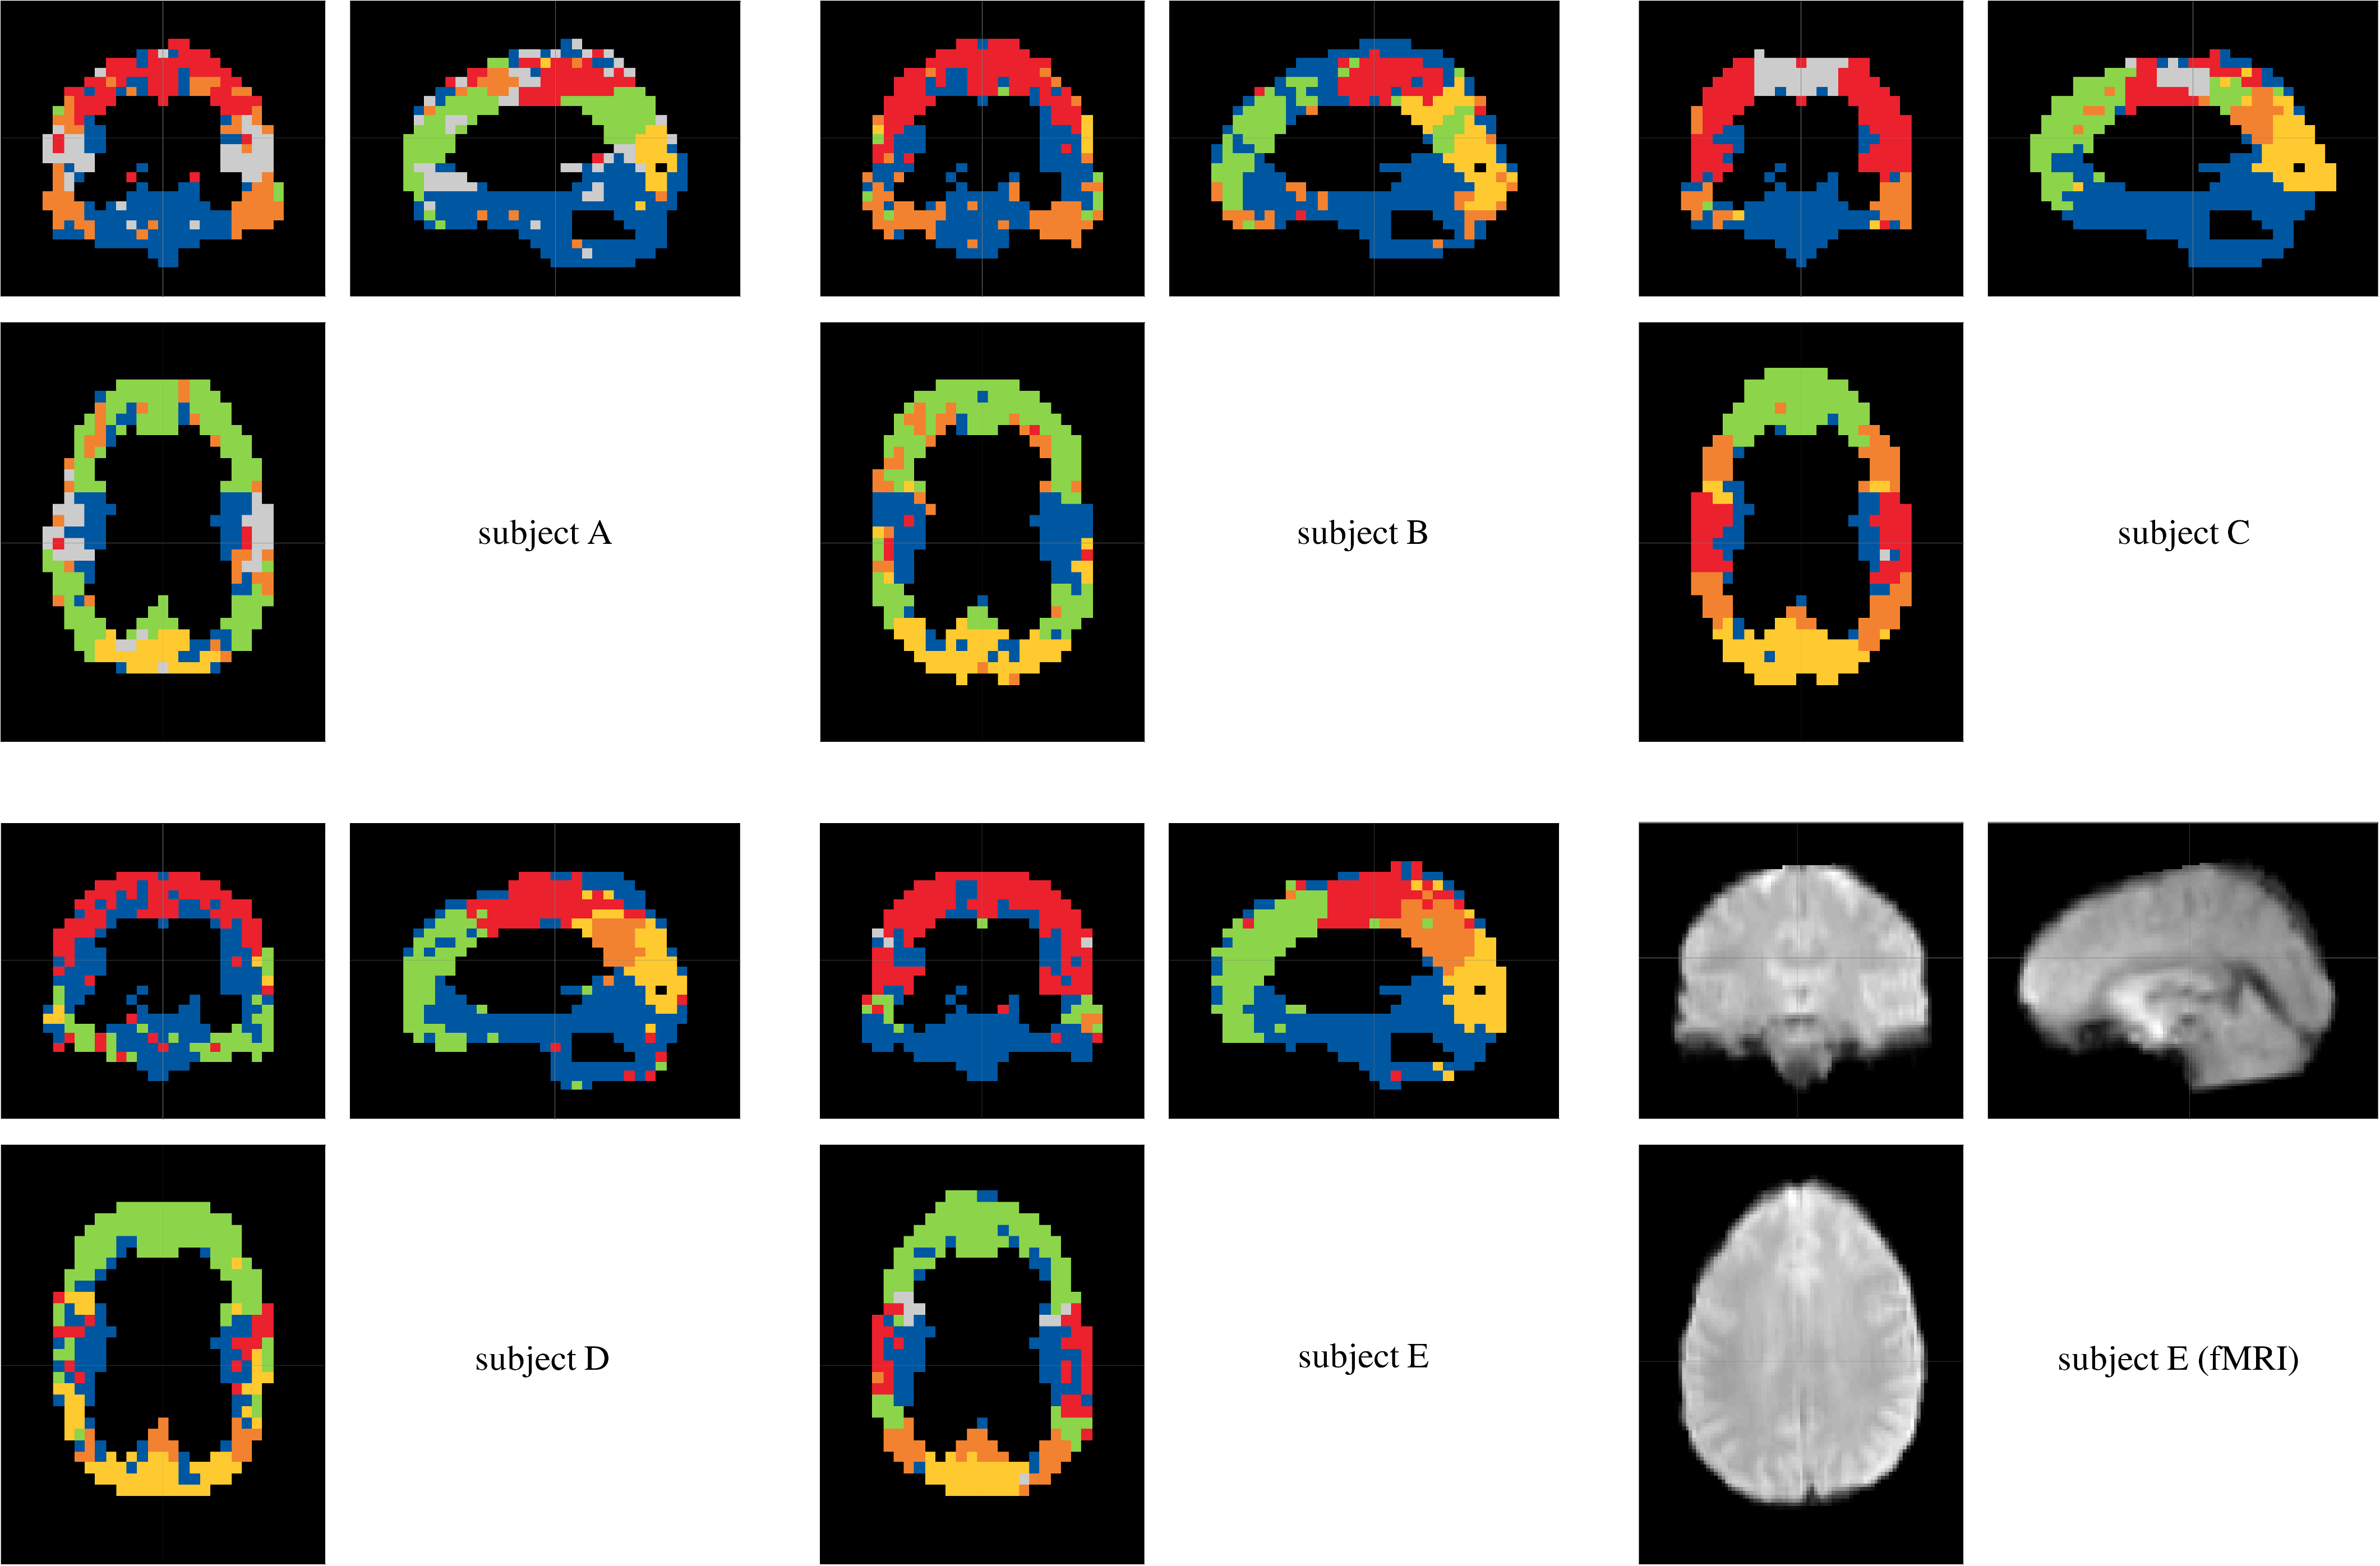
\includegraphics[width=80mm]{functional-seg-fmri.png}
  \caption{Results of functional segmentation on fMRI scan~\cite{schmidt2016multivariate}}
  \label{funcsegfMRI}
\end{figure}


\subsubsection{Physical System Description} \label{sec_phySystDescrip}

The physical system description of how fMRI scans are developed is outside the scope
of the project. We do not need to know the physical system details in order to build
the project software.

\subsubsection{Goal Statements}


\noindent Given the 4D fMRI brain scan in NIfTI format which consists of 3D brain
volumes across the time span of the scan, the goal statements are:


\begin{itemize}

  \item[GS\refstepcounter{goalnum}\thegoalnum \label{GS1}:] Visualize the 3D volume across time.
  \item[GS\refstepcounter{goalnum}\thegoalnum \label{GS2}:] Visualize 2D slice views
        (sagittal, axial, coronal) across time.
  \item[GS\refstepcounter{goalnum}\thegoalnum \label{GS3}:] Perform anatomical segmentation
        on 3D volume.
  \item[GS\refstepcounter{goalnum}\thegoalnum \label{GS4}:] Visualize the segmentation results
        in 2D slice views (sagittal, axial, coronal) across time.

\end{itemize}

\subsection{Solution Characteristics Specification}

This section provides the assumptions, data definitions, theoretical models,
instance models, and data constraints required for a successful implementation of the project.
The information in this section is provided to express the project in clear mathematical and
logical terms to remove to prevent ambiguity of the project.

The instance models that govern BrainInsight3D are presented in
Subsection~\ref{sec_instance}.  The information to understand the meaning of the
instance models and their derivation is also presented, so that the instance
models can be verified.


\subsubsection{Assumptions} \label{sec_assumpt}

\begin{itemize}

  \item[A\refstepcounter{assumpnum}\theassumpnum \label{A1}:] The user provides fMRI scans of the brain and not other organ.
  \item[A\refstepcounter{assumpnum}\theassumpnum \label{A2}:] The user provides 4D fMRI brain scans in NIfTI format.
  \item[A\refstepcounter{assumpnum}\theassumpnum \label{A3}:] The scans provided are not corrupt.
  \item[A\refstepcounter{assumpnum}\theassumpnum \label{A4}:] The metadata of the provided scans is correct.


\end{itemize}

\subsubsection{Theoretical Models}\label{sec_theoretical}

This section focuses on the general equations and laws that BrainInsight3D is based
on.

% TM1**********************%
~\newline

\noindent
\begin{minipage}{\textwidth}
  \renewcommand*{\arraystretch}{1.5}
  \begin{tabular}{| p{\colAwidth} | p{\colBwidth}|}
    \hline
    \rowcolor[gray]{0.9}
    Number   & TM\refstepcounter{theorynum}\thetheorynum \label{TM1}                                                                                      \\
    \hline
    Label    & \bf Dice Score                                                                                                                             \\
    \hline
    Symbol   & DSC                                                                                                                                        \\
    \hline
    Units    & dimensionless                                                                                                                              \\
    \hline
    Equation & $DSC = \frac{2|Y \cap \hat{Y}|}{|Y| + |\hat{Y}|} = \frac{2TP}{FP + 2TP + FN} = 2 \times \frac{precision \times recall}{precision + recall}
    $                                                                                                                                                     \\
    \hline
    Description
             & Dice score is used in image segmentation to quantify the overlap between the predicted
    segmentation and the ground truth (actual) segmentation.  A Dice score of 1 indicates perfect
    agreement between the predicted and the actual segmentation, while a score of 0 indicates no agreement.                                               \\
             & $Y$ is the set of pixels which represent ground truth segmentation.                                                                        \\
             & $\hat{Y}$ is the set of pixels which represent the predicted segmentation.                                                                 \\
             & $FP$ represents False Positives. The number of pixels that are not part of the
    segmentation in the ground truth but are incorrectly predicted as part of the segmentation by the algorithm.                                          \\
             & $FN$ represents False Negatives. The number of pixels that are part of the segmentation in the ground
    truth but are not predicted as part of the segmentation.                                                                                              \\
             & $TP$ represents True Positives. The number of pixels correctly identified as part of the segmentation.                                     \\
             & $Precision$ is the proportion of the predicted segmentation that is correct. It's calculated as
    $\frac{TP}{TP + FP }$                                                                                                                                 \\
             & $Recall$ is the proportion of the ground truth segmentation that was predicted correctly by the algorithm.
    It's calculated as $\frac{TP}{TP + FN }$                                                                                                              \\
    \hline
    Notes    & -                                                                                                                                          \\
    \hline
    Sources  & \cite{fedorov2017end}                                                                                                                      \\
    \hline
    Ref.\ By & \ddref{DD_signalImage}                                                                                                                     \\
    \hline
  \end{tabular}
\end{minipage}\\

% TM2**********************%
~\newline
\noindent
\begin{minipage}{\textwidth}
  \renewcommand*{\arraystretch}{1.5}
  \begin{tabular}{| p{\colAwidth} | p{\colBwidth}|}
    \hline
    \rowcolor[gray]{0.9}
    Number   & TM\refstepcounter{theorynum}\thetheorynum \label{TM2}                                                    \\
    \hline
    Label    & \bf Average Volume Difference                                                                            \\
    \hline
    Symbol   & AVD                                                                                                      \\
    \hline
    Units    & dimensionless                                                                                            \\
    \hline
    Equation & $AVD = \frac{2|V_P \cap V_G |}{V_G}$                                                                     \\
    \hline
    Description
             & Average Volume Difference (AVD) is used image segmentation to quantify the overlap between the predicted
    segmentation and the ground truth (actual) segmentation between volumes of data.                                    \\
             & $V_P$ is the volume of segmentation predicted by the algorithm.                                          \\
             & $V_G$ is the ground truth volume of segmentation.                                                        \\
    \hline
    Notes
             & In the context of this project, AVD can be used to compare volumes of tissues inside the brain.          \\
    \hline
    Sources  & \cite{fedorov2017end}                                                                                    \\
    \hline
    Ref.\ By & \ddref{DD_signalImage}, \tref{T_contrast}, \aref{A_yield}                                                \\
    \hline
  \end{tabular}
\end{minipage}\\


% TM3**********************%
~\newline
\noindent
\begin{minipage}{\textwidth}
  \renewcommand*{\arraystretch}{1.5}
  \begin{tabular}{| p{\colAwidth} | p{\colBwidth}|}
    \hline
    \rowcolor[gray]{0.9}
    Number   & TM\refstepcounter{theorynum}\thetheorynum \label{TM3}                                                                          \\
    \hline
    Label    & \bf Convolution                                                                                                                \\
    \hline
    Symbol   & -                                                                                                                              \\
    \hline
    Units    & dimensionless                                                                                                                  \\
    \hline
    Equation & -                                                                                                                              \\
    \hline
    Description
             & \\                                                                            \\
    \hline
    Notes
             & \\
    \hline
    Sources  & \cite{}                                                                                                           \\
    \hline
    Ref.\ By & \ddref{}, \tref{}, \aref{}                                                                      \\
    \hline
  \end{tabular}
\end{minipage}\\

% TM4**********************%
~\newline
\noindent
\begin{minipage}{\textwidth}
  \renewcommand*{\arraystretch}{1.5}
  \begin{tabular}{| p{\colAwidth} | p{\colBwidth}|}
    \hline
    \rowcolor[gray]{0.9}
    Number   & TM\refstepcounter{theorynum}\thetheorynum \label{TM4}                                                                          \\
    \hline
    Label    & \bf Kernel                                                                                                                     \\
    \hline
    Symbol   & -                                                                                                                              \\
    \hline
    Units    & dimensionless                                                                                                                  \\
    \hline
    Equation & -                                                                                                                              \\
    \hline
    Description
             & \\                                                                              \\
    \hline
    Notes
             &                               \\
    \hline
    Sources  & \cite{}                                                                                                           \\
    \hline
    Ref.\ By & \ddref{}, \tref{}, \aref{}                                                                      \\
    \hline
  \end{tabular}
\end{minipage}\\

% TM5**********************%
~\newline
\noindent
\begin{minipage}{\textwidth}
  \renewcommand*{\arraystretch}{1.5}
  \begin{tabular}{| p{\colAwidth} | p{\colBwidth}|}
    \hline
    \rowcolor[gray]{0.9}
    Number   & TM\refstepcounter{theorynum}\thetheorynum \label{TM5}                                                                          \\
    \hline
    Label    & \bf Convolutional layer                                                                                                        \\
    \hline
    Symbol   & -                                                                                                                              \\
    \hline
    Units    & dimensionless                                                                                                                  \\
    \hline
    Equation & -                                                                                                                              \\
    \hline
    Description
             &                                                                               \\
    \hline
    Notes
             &                             \\
    \hline
    Sources  & \cite{}                                                                                                           \\
    \hline
    Ref.\ By & \ddref{}, \tref{}, \aref{}                                                                      \\
    \hline
  \end{tabular}
\end{minipage}\\

\subsubsection{General Definitions}\label{sec_gendef}

There are no general definitions in this project.

\subsubsection{Data Definitions}\label{sec_datadef}

This section collects and defines all the data needed to build the instance
models. The dimension of each quantity is also given.

% DD1**********************%
~\newline

\noindent
\begin{minipage}{\textwidth}
  \renewcommand*{\arraystretch}{1.5}
  \begin{tabular}{| p{\colAwidth} | p{\colBwidth}|}
    \hline
    \rowcolor[gray]{0.9}
    Number      & DD\refstepcounter{datadefnum}\thedatadefnum \label{DD1}                     \\
    \hline
    Label       & \bf    Pixel                                                                \\
    \hline
    Symbol      & $p:\mathbb{R}$                                                              \\
    \hline
    % Units& $Mt^{-3}$\\
    % \hline
    SI Units    & -                                                                           \\
    \hline
    Equation    & -                                                                           \\
    \hline
    Description & A pixel is the smallest programmable color element on a digital screen.
    Each pixel comprises a subpixel that emits a red, green and blue (RGB) color, which displays at different intensities.
    \\
    \hline
    Sources     & \href{https://www.techtarget.com/whatis/definition/pixel}{Pixel Definition}
    \\                                          \\
    \hline
    Ref.\ By    & \ddref{DD3}                                                                 \\
    \hline
  \end{tabular}
\end{minipage}\\

% DD2**********************%
~\newline

\noindent
\begin{minipage}{\textwidth}
  \renewcommand*{\arraystretch}{1.5}
  \begin{tabular}{| p{\colAwidth} | p{\colBwidth}|}
    \hline
    \rowcolor[gray]{0.9}
    Number      & DD\refstepcounter{datadefnum}\thedatadefnum \label{DD2}                                                                            \\
    \hline
    Label       & \bf Voxel                                                                                                                          \\
    \hline
    Symbol      & $v:\mathbb{R}$                                                                                                                     \\
    \hline
    % Units& $Mt^{-3}$\\
    % \hline
    SI Units    & -                                                                                                                                  \\
    \hline
    Equation    & -                                                                                                                                  \\
    \hline
    Description & A Voxel is short for volumetric pixel. A voxel is the smallest unit to represent a volume
    in 3D space. Voxels are expresed using three-dimensional coordinates (x,y,z).

    \\
    \hline
    Sources     & \href{https://blogs.scientificamerican.com/observations/whats-a-voxel-and-what-can-it-tell-us-a-primer-on-fmri/}{Voxel Definition} \\
    \hline
    Ref.\ By    & \ddref{DD4}                                                                                                                        \\
    \hline
  \end{tabular}
\end{minipage}\\

% DD3**********************%
~\newline

\noindent
\begin{minipage}{\textwidth}
  \renewcommand*{\arraystretch}{1.5}
  \begin{tabular}{| p{\colAwidth} | p{\colBwidth}|}
    \hline
    \rowcolor[gray]{0.9}
    Number      & DD\refstepcounter{datadefnum}\thedatadefnum \label{DD3}                                 \\
    \hline
    Label       & \bf Image                                                                               \\
    \hline
    Symbol      & $F(x,y) : x \in \mathbb{R}^{m \times n},  y \in \mathbb{R}^{m \times n}$                \\
    \hline
    % Units& $Mt^{-3}$\\
    % \hline
    SI Units    & -                                                                                       \\
    \hline
    Equation    & -                                                                                       \\
    \hline
    Description & An image is a mapping from the continous spatial domain to the discrete digital domain.
    An image consists of a number of pixels (DD\ref*{DD1}).

    \\
    \hline
    Sources     & \href{https://ai.stanford.edu/~syyeung/cvweb/tutorial1.html}{Image Definition}          \\
    \hline
    Ref.\ By    & \ddref{ewat}                                                                             \\
    \hline
  \end{tabular}
\end{minipage}\\

% DD4**********************%

~\newline

\noindent
\begin{minipage}{\textwidth}
  \renewcommand*{\arraystretch}{1.5}
  \begin{tabular}{| p{\colAwidth} | p{\colBwidth}|}
    \hline
    \rowcolor[gray]{0.9}
    Number      & DD\refstepcounter{datadefnum}\thedatadefnum \label{DD4}                                                    \\
    \hline
    Label       & \bf Volume                                                                                                 \\
    \hline
    Symbol      & $F(x,y,z) : x \in \mathbb{R}^{m \times n},  y \in \mathbb{R}^{m \times n},  z \in \mathbb{R}^{m \times n}$ \\
    \hline
    % Units& $Mt^{-3}$\\
    % \hline
    SI Units    & -                                                                                                          \\
    \hline
    Equation    & -                                                                                                          \\
    \hline
    Description & A Volume is a grid based representation of 3D spaces. It consists of
    an array of voxels DD\ref*{DD3}.

    \\
    \hline
    Sources     & -                                                                                            \\
    \hline
    Ref.\ By    & -                                                                                              \\
    \hline
  \end{tabular}
\end{minipage}\\



\subsubsection{Instance Models} \label{sec_instance}



~\newline

%Instance Model 1

\noindent
\begin{minipage}{\textwidth}
  \renewcommand*{\arraystretch}{1.5}
  \begin{tabular}{| p{\colAwidth} | p{\colBwidth}|}
    \hline
    \rowcolor[gray]{0.9}
    Number      & IM\refstepcounter{instnum}\theinstnum \label{IM1}                                   \\
    \hline
    Label       & \bf Segmentation                                                                    \\
    \hline
    Input       & 3D volume in 3D segmentation, 2D slice/image in 2D segmentation.                                                        \\
                     \\
    \hline
    Output      & Segmented Volume (Voxels are labeled) in 3D segmentation. Segmented Slice/Image (Pixels are labeled) in 2D segmentation.\\
    \hline
    Description & Segmentation precisely divides an object into related entities, each representing specific locations or meanings. 
    In medical imaging there exist two types of segmentation: functional segmentation, which focuses on brain activity, 
    and anatomical segmentation, which details the brain's physical structure.
    \\
    \hline
    Sources     & -                                                                    \\
    \hline
    Ref.\ By    & \iref{IM2}                                                                         \\
    \hline
  \end{tabular}
\end{minipage}\\


% Instance Model 2
~\newline

\noindent
\begin{minipage}{\textwidth}
  \renewcommand*{\arraystretch}{1.5}
  \begin{tabular}{| p{\colAwidth} | p{\colBwidth}|}
    \hline
    \rowcolor[gray]{0.9}
    Number      & IM\refstepcounter{instnum}\theinstnum \label{IM2}                                   \\
    \hline
    Label       & \bf Anatomical Segmentation                                                         \\
    \hline
    Input       & 3D volume in 3D segmentation, 2D slice/image in 2D segmentation.                                                        \\
    \hline
    Output      & Segmented Volume into tissues (Voxels are labeled to belong to a certain tissue) in 3D segmentation. Segmented Slice/Image (Pixels are labeled) in 2D segmentation.\\
    \hline
    Description & Asubset of segmentation IM\ref*{IM1}. A process that divides the brain into structurally distinct areas based on MRI scans,
    identifying regions such as gray matter, white matter, and cerebrospinal fluid.
    \\
    \hline
    Sources     & -                                                                    \\
    \hline
    Ref.\ By    & -                                                                       \\
    \hline
  \end{tabular}
\end{minipage}\\



\subsubsection{Input Data Constraints} \label{sec_DataConstraints}

The only input data constraint is that the input data must be in NIfTI format. There will be
preprocessing steps in the project's algorithm to resize and resample the scan volume to 256x256x256 volumes
with 1x1x1 mm voxels for input to the segmentation algorithm.
\subsubsection{Properties of a Correct Solution} \label{sec_CorrectSolution}

\noindent
A correct solution must provide visually clear visualization of fMRI scans and segmentation results
where each brain area is color coded and the colors are visually differentiable. The solution must allow
the user to view different 2D slices and 3D volumes and sub-volumes at various time points.

\section{Requirements}

This section provides the functional requirements, the business tasks that the
software is expected to complete, and the nonfunctional requirements, the
qualities that the software is expected to exhibit.

\subsection{Functional Requirements}

\noindent \begin{itemize}

  \item[R\refstepcounter{reqnum}\thereqnum \label{R1}:] The system should allow the users
        to input 4D scans with the associated metadata in the supported formats(NIfTI).

  \item[R\refstepcounter{reqnum}\thereqnum \label{R2}:] The system should clearly
        output a visualization of 3D volume and 2D slices in the coronal, sagittal, and axial views
        of the input fMRI scan.

  \item[R\refstepcounter{reqnum}\thereqnum \label{R3}:]The system should enable the user
        to navigate through different time points for 2D slice views and 3D volumes.

  \item[R\refstepcounter{reqnum}\thereqnum \label{R4}:]The system should provide functionality for
        users to navigate through time points and view the segmentation results at each point in time

  \item[R\refstepcounter{reqnum}\thereqnum \label{R5}:] The system should perform all required data preprocessing
        to accurately visualize input data \ref*{R2} and perform segmentation \ref*{IM2} \ref*{R4}

  \item[R\refstepcounter{reqnum}\thereqnum \label{R6}:] The system should implement an algorithm or
        set of algorithms capable of performing anatomical segmentation on 3D volumes \ref{IM1} \ref*{IM2}.


\end{itemize}



\subsection{Nonfunctional Requirements}

\noindent \begin{itemize}

  \item[NFR\refstepcounter{nfrnum}\thenfrnum \label{NFR_Accuracy}:]
        \textbf{Accuracy}: The segmentation accuracy should be comparable with the most up to date benchmarks for brain anatomical segmentation.

  \item[NFR\refstepcounter{nfrnum}\thenfrnum \label{NFR_Usability}:] \textbf{Usability}: The system should offer a user inferface that is easy to use with minimal
        training by both experts and general users.


  \item[NFR\refstepcounter{nfrnum}\thenfrnum \label{NFR_Maintainability}:]
        \textbf{Maintainability}: The system should be implemented in a manner that enables improvements to current functionality and smooth addition of new functionalities

  \item[NFR\refstepcounter{nfrnum}\thenfrnum \label{NFR_Portability}:]
        \textbf{Portability}: The system should work on any device with modern browser. Users shouldn't have to install any dependencies for the system to work.

\end{itemize}
Other NFRs that might be discussed include verifiability,understandability
and reusability.

\section{Likely Changes}

\noindent \begin{itemize}

  \item[LC\refstepcounter{lcnum}\thelcnum\label{LC1}:] The algorithm used for the segmentation can change
        after experimentation and evaluation of accuracy and speed of inference.
  \item[LC\refstepcounter{lcnum}\thelcnum\label{LC2}:] The visualization steps order and algorithms can change after
        experimentation to achieve the best visualization output.

\end{itemize}

\section{Unlikely Changes}

\noindent \begin{itemize}

  \item[ULC\refstepcounter{ulcnum}\thelcnum\label{ULC1}:] The project is unlikely to cover
        functional segmentation.

\end{itemize}

\section{Traceability Matrices and Graphs}

The purpose of the traceability matrices is to provide easy references on what
has to be additionally modified if a certain component is changed.  Every time a
component is changed, the items in the column of that component that are marked
with an ``X'' may have to be modified as well.  Table~\ref{Table:trace} shows the
dependencies of theoretical models, general definitions, data definitions, and
instance models with each other. Table~\ref{Table:R_trace} shows the
dependencies of instance models, requirements, and data constraints on each
other. Table~\ref{Table:A_trace} shows the dependencies of theoretical models,
general definitions, data definitions, instance models, and likely changes on
the assumptions.


\afterpage{
  \begin{landscape}
    \begin{table}[h!]
      \centering
      \begin{tabular}{|c|c|c|c|c|c|c|c|c|c|c|c|c|c|c|c|c|c|c|c|}
        \hline
                            & \aref{A1} & \aref{A2} & \aref{A3} & \aref{A4}  \\
        \hline
        \tref{TM1}        & X                          &                 &                &             \\ \hline
        \tref{TM2}        &                            &                 &                &                  \\ \hline
        \tref{TM3}        &                            &                 &                &                \\ \hline
        \dref{TM4}           &                            & X               &                &                    \\ \hline
        \dref{TM5}         &                            &                 & X              & X              \\ \hline
        \ddref{DD1}    &                            &                 &                &                          \\ \hline
        \ddref{DD2}     &                            &                 & X              & X                        \\ \hline
        \ddref{DD3}       &                            &                 &                &                          \\ \hline
        \ddref{DD4}        &                            &                 &                &                          \\ \hline
        \iref{IM1}         &                            &                 &                &                          \\ \hline
        \iref{IM2}         &                            &                 &                &                          \\ \hline
        \lcref{LC1}     &                            &                 &                & X                        \\ \hline
        \lcref{LC2}    &                            &                 &                &                          \\ \hline
        \lcref{ULC1}   &                            &                 &                &                          \\ \hline
       \hline
      \end{tabular}
      \caption{Traceability Matrix Showing the Connections Between Assumptions and Other Items}
      \label{Table:A_trace}
    \end{table}
  \end{landscape}
}

\begin{table}[h!]
  \centering
  \begin{tabular}{|c|c|c|c|c|c|c|c|c|c|c|c|c|c|c|c|c|c|c|c|c|c|c|c|}
    \hline
                     & \tref{T_COE} & \tref{T_SHE} & \tref{T_LHE} & \dref{NL} & \dref{ROCT} & \ddref{FluxCoil} & \ddref{FluxPCM} & \ddref{D_HOF} & \ddref{D_MF} & \iref{ewat} & \iref{epcm} & \iref{I_HWAT} & \iref{I_HPCM} \\
    \hline
    \tref{TM1}     &              &              &              &           &             &                  &                 &               &              &             &             &               &               \\ \hline
    \tref{TM2}     &              &              & X            &           &             &                  &                 &               &              &             &             &               &               \\ \hline
    \tref{TM3}     &              &              &              &           &             &                  &                 &               &              &             &             &               &               \\ \hline
    \dref{TM4}        &              &              &              &           &             &                  &                 &               &              &             &             &               &               \\ \hline
    \dref{TM5}      & X            &              &              &           &             &                  &                 &               &              &             &             &               &               \\ \hline
    \ddref{FluxCoil} &              &              &              & X         &             &                  &                 &               &              &             &             &               &               \\ \hline
    \ddref{FluxPCM}  &              &              &              & X         &             &                  &                 &               &              &             &             &               &               \\ \hline
    \ddref{D_HOF}    &              &              &              &           &             &                  &                 &               &              &             &             &               &               \\ \hline
    \ddref{D_MF}     &              &              &              &           &             &                  &                 & X             &              &             &             &               &               \\ \hline
    \iref{ewat}      &              &              &              &           & X           & X                & X               &               &              &             & X           &               &               \\ \hline
    \iref{epcm}      &              &              &              &           & X           &                  & X               &               & X            & X           &             &               & X             \\ \hline
    \iref{I_HWAT}    &              & X            &              &           &             &                  &                 &               &              &             &             &               &               \\ \hline
    \iref{I_HPCM}    &              & X            & X            &           &             &                  & X               & X             & X            &             & X           &               &               \\
    \hline
  \end{tabular}
  \caption{Traceability Matrix Showing the Connections Between Items of Different Sections}
  \label{Table:trace}
\end{table}

\begin{table}[h!]
  \centering
  \begin{tabular}{|c|c|c|c|c|c|c|c|}
    \hline
                           & \iref{IM1} & \iref{IM2}  & \rref{R1} & \rref{R2} & \rref{R3} & \rref{R4} & \rref{R5} & \rref{R6} \\
    \hline
    \iref{IM1}            &             & X           &      X         &    X           &                           &              & X         & X         \\ \hline
    \iref{IM2}            & X           &             &               & X             &                           & X                  &    X     & X           \\ \hline
    \rref{R1}     &           X  &             &               &               &                           &            X        &              &              \\ \hline
    \rref{R2}    &           X  &  X           &               &               &                           & X                  &             &               \\ \hline
    \rref{R3}   &             &             &               &               & X                         &                    &             &               \\ \hline
    \rref{R4}  &     &            &     X          &               &                           &                  &             &              \\ \hline
    \rref{R5}     & X           &             &               &               &                           &                    &            &                \\ \hline
    \rref{R6}       &   X          & X           &               &               &                           &                    &          &                  \\ \hline
  \end{tabular}
  \caption{Traceability Matrix Showing the Connections Between Requirements and Instance Models}
  \label{Table:R_trace}
\end{table}

The purpose of the traceability graphs is also to provide easy references on
what has to be additionally modified if a certain component is changed.  The
arrows in the graphs represent dependencies. The component at the tail of an
arrow is depended on by the component at the head of that arrow. Therefore, if a
component is changed, the components that it points to should also be
changed. Figure~\ref{Fig_ATrace} shows the dependencies of theoretical models,
general definitions, data definitions, instance models, likely changes, and
assumptions on each other. Figure~\ref{Fig_RTrace} shows the dependencies of
instance models, requirements, and data constraints on each other.


\newpage

\bibliographystyle {plainnat}
\bibliography {../../refs/References}



\end{document}